% Adjust these for the path of the theme and its graphics, relative to this file
%\usepackage{beamerthemeFalmouthGamesAcademy}
\usepackage{../../beamerthemeFalmouthGamesAcademy}
\usepackage{multimedia}
\graphicspath{ {../../} }

% Default language for code listings
\lstset{language=C++,
        morekeywords={each,in,nullptr}
}

% From http://blog.virtualglobebook.com/2011/02/syntax-highlighting-c-and-glsl-source.html

\lstdefinelanguage{GLSL}
{
sensitive=true,
morekeywords=[1]{
attribute, const, uniform, varying,
layout, centroid, flat, smooth,
noperspective, break, continue, do,
for, while, switch, case, default, if,
else, in, out, inout, float, int, void,
bool, true, false, invariant, discard,
return, mat2, mat3, mat4, mat2x2, mat2x3,
mat2x4, mat3x2, mat3x3, mat3x4, mat4x2,
mat4x3, mat4x4, vec2, vec3, vec4, ivec2,
ivec3, ivec4, bvec2, bvec3, bvec4, uint,
uvec2, uvec3, uvec4, lowp, mediump, highp,
precision, sampler1D, sampler2D, sampler3D,
samplerCube, sampler1DShadow,
sampler2DShadow, samplerCubeShadow,
sampler1DArray, sampler2DArray,
sampler1DArrayShadow, sampler2DArrayShadow,
isampler1D, isampler2D, isampler3D,
isamplerCube, isampler1DArray,
isampler2DArray, usampler1D, usampler2D,
usampler3D, usamplerCube, usampler1DArray,
usampler2DArray, sampler2DRect,
sampler2DRectShadow, isampler2DRect,
usampler2DRect, samplerBuffer,
isamplerBuffer, usamplerBuffer, sampler2DMS,
isampler2DMS, usampler2DMS,
sampler2DMSArray, isampler2DMSArray,
usampler2DMSArray, struct},
morekeywords=[2]{
radians,degrees,sin,cos,tan,asin,acos,atan,
atan,sinh,cosh,tanh,asinh,acosh,atanh,pow,
exp,log,exp2,log2,sqrt,inversesqrt,abs,sign,
floor,trunc,round,roundEven,ceil,fract,mod,modf,
min,max,clamp,mix,step,smoothstep,isnan,isinf,
floatBitsToInt,floatBitsToUint,intBitsToFloat,
uintBitsToFloat,length,distance,dot,cross,
normalize,faceforward,reflect,refract,
matrixCompMult,outerProduct,transpose,
determinant,inverse,lessThan,lessThanEqual,
greaterThan,greaterThanEqual,equal,notEqual,
any,all,not,textureSize,texture,textureProj,
textureLod,textureOffset,texelFetch,
texelFetchOffset,textureProjOffset,
textureLodOffset,textureProjLod,
textureProjLodOffset,textureGrad,
textureGradOffset,textureProjGrad,
textureProjGradOffset,texture1D,texture1DProj,
texture1DProjLod,texture2D,texture2DProj,
texture2DLod,texture2DProjLod,texture3D,
texture3DProj,texture3DLod,texture3DProjLod,
textureCube,textureCubeLod,shadow1D,shadow2D,
shadow1DProj,shadow2DProj,shadow1DLod,
shadow2DLod,shadow1DProjLod,shadow2DProjLod,
dFdx,dFdy,fwidth,noise1,noise2,noise3,noise4,
EmitVertex,EndPrimitive},
morekeywords=[3]{
gl_VertexID,gl_InstanceID,gl_Position,
gl_PointSize,gl_ClipDistance,gl_PerVertex,
gl_Layer,gl_ClipVertex,gl_FragCoord,
gl_FrontFacing,gl_ClipDistance,gl_FragColor,
gl_FragData,gl_MaxDrawBuffers,gl_FragDepth,
gl_PointCoord,gl_PrimitiveID,
gl_MaxVertexAttribs,gl_MaxVertexUniformComponents,
gl_MaxVaryingFloats,gl_MaxVaryingComponents,
gl_MaxVertexOutputComponents,
gl_MaxGeometryInputComponents,
gl_MaxGeometryOutputComponents,
gl_MaxFragmentInputComponents,
gl_MaxVertexTextureImageUnits,
gl_MaxCombinedTextureImageUnits,
gl_MaxTextureImageUnits,
gl_MaxFragmentUniformComponents,
gl_MaxDrawBuffers,gl_MaxClipDistances,
gl_MaxGeometryTextureImageUnits,
gl_MaxGeometryOutputVertices,
gl_MaxGeometryOutputVertices,
gl_MaxGeometryTotalOutputComponents,
gl_MaxGeometryUniformComponents,
gl_MaxGeometryVaryingComponents,gl_DepthRange},
morecomment=[l]{//},
morecomment=[s]{/*}{*/},
morecomment=[l][keywordstyle4]{\#},
}


% For strikethrough effect
\usepackage[normalem]{ulem}
\usepackage{wasysym}

\usepackage{pdfpages}

\usepackage{caption}
\captionsetup[figure]{font=scriptsize,labelfont=scriptsize}

% http://www.texample.net/tikz/examples/state-machine/
\usetikzlibrary{arrows,automata}

\newcommand{\modulecode}{COMP260}\newcommand{\moduletitle}{Distributed Systems}\newcommand{\sessionnumber}{5}

\begin{document}
\title{\sessionnumber: Textures \& Models}
\subtitle{\modulecode: \moduletitle}

\frame{\titlepage} 

\begin{frame}{Worksheet Schedule}
	\begin{center}
		\begin{tabular}{|l l l|}
			\hline
			\textbf{Worksheet} & \textbf{Start} & \textbf{Formative deadline} \\
			\hline
			\textbf{1}: Framework & Week 2 & Mon \textbf{15th Feb} 4pm (Week 4) \\
			\hline
			\textbf{2}: Basic scene & Week 4 & Mon \textbf{1st Mar} 4pm (Week 6) \\
			\hline
			\textbf{3}: Plan/prototype & Week 6 & Mon \textbf{15th Mar} 4pm (Week 8) \\
			\hline
			\textbf{4}: Final iteration & Week 8 & Mon \textbf{12th Apr} 4pm (Week 10) \\
			\hline
		\end{tabular}
	\end{center}
\end{frame}


\begin{frame}{Learning outcomes}
	By the end of this week, you should be able to:
	\begin{itemize}
		\item \textbf{Recall} alternative ways to represent mesh vertices in memory.
		\item \textbf{Apply} basic transforms using the GLM library.
		\item \textbf{Explain} the constituents of the model-view-projection matrix and how it can be used to create a first-person camera controller.
	\end{itemize}
\end{frame}

\begin{frame}{Agenda}
	\begin{itemize}
		\pause\item Lecture (async):
		\begin{itemize}
			\item \textbf{Compare} different ways to store vertex data in memory.
			\item \textbf{Review} the transforms required to display 3D objects on a 2D screen.
		\end{itemize}
		\pause\item Workshop (sync):
		\begin{itemize}
			\item \textbf{Adapt} our basic triangle implementation to draw meshes with multiple triangles efficiently.
			\item \textbf{Experiment} with creating transforms using GLM and using them to move objects and the camera.
		\end{itemize}
	\end{itemize}
\end{frame}

\begin{frame}{Schedule}
	\begin{center}
		\begin{tabular}{|c c|}
			\hline
			16:00-16:10 & Arrival, sign-in \& overview \\
			\hline
			16:10-16:40 & Demo \& Exercise: Loading Textures \\
			\hline
			16:40-16:50 & Introduction to Assimp\\
			16:50-17:30 & Demo \& Exercise: Loading a Mesh from File \\
			17:30-18:00 & Parsing a Scene and Storing Data \\
			\hline
		\end{tabular}
	\end{center}
\end{frame}

\part{Applying textures in OpenGL}
\frame{\partpage}

\begin{frame}[fragile]{Texture loading}
	\pause Load with SDL Image:
	\begin{lstlisting}
SDL_Surface* image = IMG_Load("Crate.jpg");
	\end{lstlisting}
	\pause Set up in OpenGL:
	\begin{lstlisting}
GLuint textureID;
glGenTextures(1, &textureID);
glBindTexture(GL_TEXTURE_2D, textureID);
glTexImage2D(GL_TEXTURE_2D, 0, GL_RGB, image->w, image->h,
			0, GL_RGB, GL_UNSIGNED_BYTE, image->pixels);
	\end{lstlisting}
	\pause Assign texture coordinates to each vertex - as for any other attribute.
\end{frame}

\begin{frame}[fragile]{Texture filtering}
	\begin{lstlisting}
glTexParameteri(GL_TEXTURE_2D, GL_TEXTURE_MIN_FILTER,
				GL_LINEAR);
glTexParameteri(GL_TEXTURE_2D, GL_TEXTURE_MAG_FILTER,
				GL_LINEAR);
	\end{lstlisting}
	\begin{itemize}
		\pause\item \textbf{Linear interpolation} (\lstinline{GL_LINEAR})
			smooths between pixels
		\pause\item \textbf{Nearest neighbour} (\lstinline{GL_NEAREST})
			is pixelated but may be slightly faster
		\pause\item \textbf{Mip-mapping} pre-calculates scaled down versions of the texture ---
			improves quality but costs memory
	\end{itemize}
	\pause \begin{lstlisting}
glGenerateMipmap(GL_TEXTURE_2D);
	\end{lstlisting}
\end{frame}

\begin{frame}[fragile]{Textures in GLSL}
	Fragment shader:
	
	\begin{lstlisting}[language=GLSL]
in vec2 textureCoords;
uniform sampler2D textureSampler;

void main()
{
    fragmentColour = texture(textureSampler, textureCoords);
}
	\end{lstlisting}
\end{frame}

\begin{frame}[fragile]{Alpha in OpenGL}
	\begin{itemize}
		\item Use \lstinline[language=GLSL]{vec4} instead of \lstinline[language=GLSL]{vec3} for colours
		\pause\item Textures can have an \textbf{alpha channel}
			\begin{itemize}
				\pause\item PNG supports alpha channels, JPG and BMP do not
			\end{itemize}
		\pause\item Need to enable \textbf{alpha blending}
	\end{itemize}
	\pause
	\begin{lstlisting}
glEnable(GL_BLEND);
glBlendFunc(GL_SRC_ALPHA, GL_ONE_MINUS_SRC_ALPHA);
	\end{lstlisting}
	\begin{itemize}	
		\item Other values can be passed to \lstinline{glBlendFunc} for special effects
			(e.g.\ \textbf{additive blending} is often used for particle effects simulating
				light, fire, explosions etc.)
	\end{itemize}
\end{frame}

\part{Importing models}
\frame{\partpage}

\begin{frame}{Open Asset Import Library}
	\begin{itemize}
		\item There is an FBX SDK published by Autodesk, this can be used to load FBX files
		\pause\item We will use Asset Import Library to load FBX files
		\pause\item This allows us to support multiple file formats, including
		\begin{itemize}
			\pause\item FBX
			\pause\item OBJ 
			\pause\item DAE (aka Collada)
			\pause\item MD5 (DOOM3)
			\pause\item SMD (Half Life 2, Portal etc)
		\end{itemize}
	\end{itemize}
\end{frame}

\begin{frame}{Overview of an Assimp scene}
	\begin{center}
		\begin{figure}[h!]
			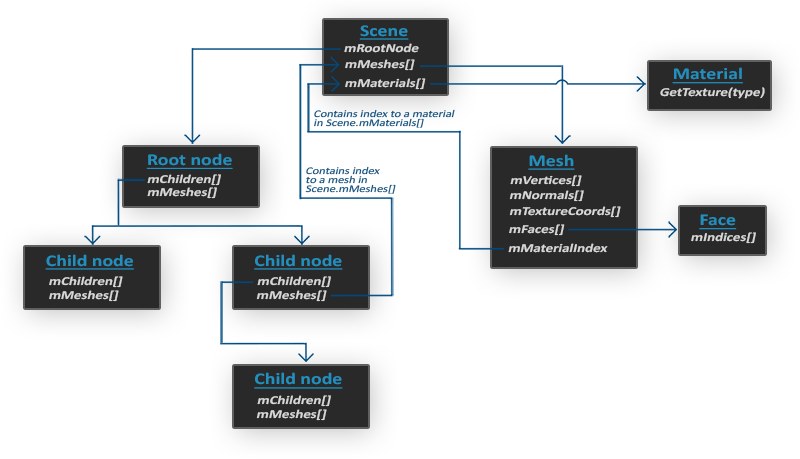
\includegraphics[width=\textwidth]{assimp_structure}
			\caption*{Image source: \url{https://learnopengl.com/Model-Loading/Assimp}}
		\end{figure}
	\end{center}
\end{frame}

\begin{frame}[fragile]{Loading a model from file}
		\begin{lstlisting}
Assimp::Importer importer;
const aiScene *scene = importer.ReadFile(path, flags); 
		\end{lstlisting}
		\begin{itemize}
		\pause\item An \href{http://assimp.sourceforge.net/lib_html/structai_scene.html}{\color{cyan}\lstinline{aiScene}} has (amongst other things):
		\begin{itemize}
			\pause\item \lstinline{aiMesh** mMeshes} - an array of pointers to the meshes in the scene
			\pause\item \lstinline{aiNode* mRootNode} - a pointer to the root node of the scene (provides access to all child nodes)
		\end{itemize}
		\pause\item An \href{http://assimp.sourceforge.net/lib_html/structai_node.html}{\color{cyan}\lstinline{aiNode}} has pointers to its \textbf{parent} and \textbf{child} nodes, the \textbf{indices} of its meshes, and a \textbf{transform} relative to its parent.
		\pause\item Optional \href{http://assimp.sourceforge.net/lib_html/postprocess_8h.html#a64795260b95f5a4b3f3dc1be4f52e410}{\color{cyan}\lstinline{flags}} can be supplied to specify post-processing steps, e.g. \lstinline{aiProcess_Triangulate}, \lstinline{aiProcess_GenNormals}
	\end{itemize} 
\end{frame}

\end{document}
